\documentclass[12pt]{article}

\usepackage[utf8]{inputenc}
\usepackage[T1]{fontenc}
\usepackage[spanish]{babel}
\usepackage{graphicx}
\usepackage{listings}
\usepackage{caption}
\usepackage{subcaption}
\usepackage[right=2cm,left=2cm,top=2cm,bottom=2cm]{geometry}
\usepackage{hyperref}
\usepackage{fancyhdr}
\usepackage{color}
\usepackage[export]{adjustbox}
\usepackage{graphicx}
\usepackage{float}
\usepackage{changepage}
\usepackage{multicol}
\usepackage{imakeidx}
\usepackage[spanish]{babel}
\usepackage[backend=biber]{biblatex}
\usepackage{amsmath}

\pagestyle{fancy}
\renewcommand{\footrulewidth}{0.4pt}
\setlength{\headheight}{15pt}


\fancyhead[L]{ CEIABD – SAA }
\fancyhead[R]{ Páez Anguita, Víctor }
\fancyfoot[L]{IES Gran Capitán}


\begin{document}

\begin{titlepage}
    \begin{center}
      \Large \bfseries{}
    \end{center}
    \vspace{0.8cm}
    \begin{center}
      \Large \bfseries{}
    \end{center}
    \vspace{0.8cm}
    \begin{center}
     \Large \bfseries{Problema de la dieta}
    \end{center}
    \vspace{0.0001cm}
    \begin{center}
        Departamento de informática \\ I.E.S. Gran Capitán - Córdoba
    \end{center}
        \vspace{2 cm}
    \vspace{0.2 cm}
    \begin{center}
        Inteligencia artificial y Big data \\ Córdoba, 20 de Octubre 2024
    \end{center}
    \vspace{10 cm}
\null\hfill \textbf{Desarrollado por:}
\\
\\
\null\hfill Víctor Páez Anguita
\clearpage
\end{titlepage}

%%%%%%%%%%%%%%%%%%%%%%%%%%%Index%%%%%%%%%%%%%%%%%%%%%%%%%%%%%%%%
\tableofcontents
\clearpage
%%%%%%%%%%%%%%%%%%%%%%%%%%%Index%%%%%%%%%%%%%%%%%%%%%%%%%%%%%%%%

\section{Problema}

\subsection{Supuesto A}

Añadimos a la dieta dos productos alimenticios más: 

\begin{itemize}
    \item Carne, precio: 5.5, proteinas: 4, calorías: 2500
    \item Huevos, precio: 0.5, proteinas: 1, calorías: 500
\end{itemize}

Y fijamos el máximo de calorías de la dieta en 5000
\\\\
Siguiendo lo siguiente nos quedaría tal que:

\begin{itemize}
    \item Variables de decisión: \( x_A, x_P, x_V, x_C, x_H \)
    \item Función objetivo: Minimizar: \( f(x_A, x_P, x_V, x_C, x_H) = 1,5x_A + 7x_P + 2,5x_V + 5,5x_C + 0,5x_H \)
    \item Restricciones: Sigue habiendo las mismas tres restricciones añadiendo el máximo de calorias. Que se cumpla los requerimientos de 
    proteina, calorias y las cantidades deben ser enteras y no negativas.
\end{itemize}

Modelo de optimización:
\\\\
Minimizar: \( f(x_A, x_P, x_V, x_C, x_H) = 1,5x_A + 7x_P + 2,5x_V + 5,5x_C + 0,5x_H\)
\\
Sujeto a: 
\begin{align*}
    x_A + 3x_P + 2x_V + 4x_C + x_H & \geq 3 \\
    2000x_A + 3000x_P + 1000x_V + 2500x_C + 500x_H & \geq 4000 \\
    2000x_A + 3000x_P + 1000x_V + 2500x_C + 500x_H & \leq 5000 \\
    x_A, x_P, x_V, x_C, x_H & \geq 0
\end{align*}

Si queremos resolverlo en excel con solver, quedaria tal que así:
\begin{figure}[h!]
    \centering
    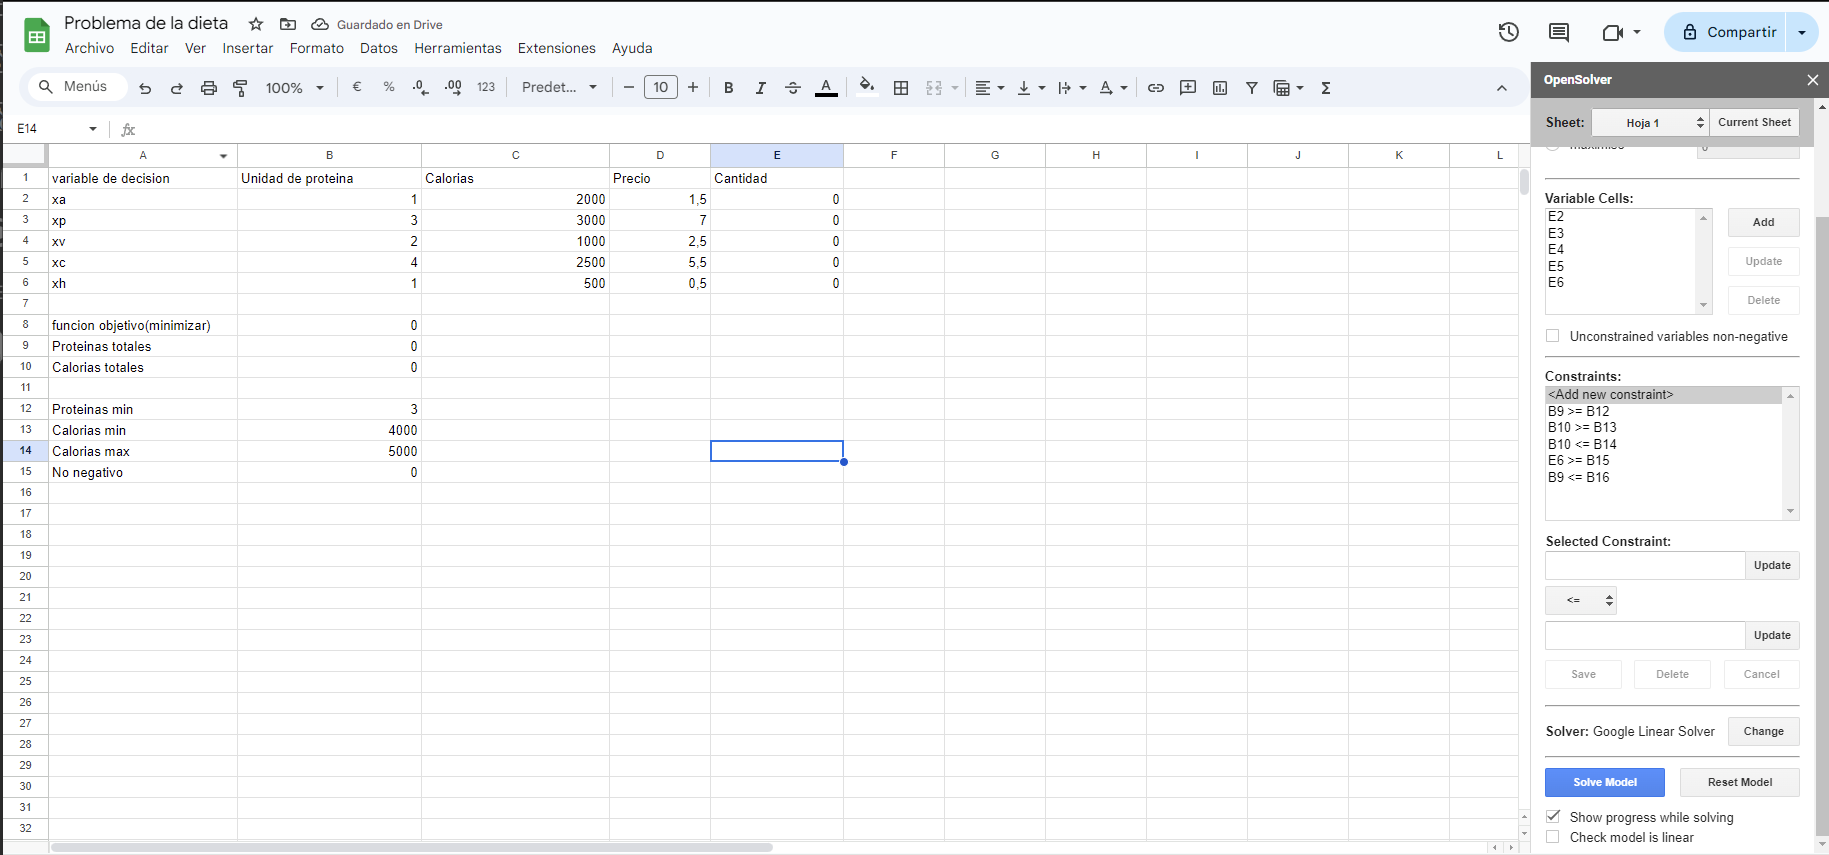
\includegraphics[width=.6\textwidth]{supuestoA.PNG}
    \label{fig:my_label}
\end{figure}

La herramienta de solver daba error, por lo que no he podido mostrar el resultado final solo el planteamiento.
\clearpage
\subsection{Supuesto B}

La dieta se va a contemplar de manera semanal, de forma que:

\begin{itemize}
    \item Mínimo de calorías: 28000
    \item Máximo de calorías: 35000
    \item Mínimo de proteínas: 28
    \item Máximo de proteínas: 50
\end{itemize}

Además hay un número mínimo que se debe consumir de cada producto:

\begin{itemize}
    \item Carne >= 1
    \item Pescado >= 1
    \item Huevos >= 2
    \item Verduras >= 1
\end{itemize}

En este caso como la dieta ha pasado a contemplarse de manera semanal, la función objetivo a minimizar queda tal que:

\begin{itemize}
    \item Función objetivo: Minimizar: \( f(x_A, x_P, x_V, x_C, x_H) = 7(1,5x_A + 7x_P + 2,5x_V + 5,5x_C + 0,5x_H) \)
\end{itemize}
Tenemos ahora un aumento de restricciones, ya que nos piden tanto mínimos como máximos por ambas partes de unidades de proteina y calorias. Además,
También han cambiado los números mínimos de alimento que se debe consumir. Por lo que nuestras restricciones quedarian:
\\
\begin{itemize}
    \item Proteínas mínimas: \( 1x_A + 3x_P + 2x_V + 4x_C + 1x_H \geq 28 \)
    \item Proteínas máximas: \( 1x_A + 3x_P + 2x_V + 4x_C + 1x_H \leq 50 \)
    \item Calorías mínimas: \( 2000x_A + 3000x_P + 1000x_V + 2500x_C + 500x_H \geq 28000 \)
    \item Calorías máximas: \( 2000x_A + 3000x_P + 1000x_V + 2500x_C + 500x_H \leq 35000 \)
    \item Consumo mínimo de ciertos productos:
    \begin{align*}
        x_C & \geq 1 \\
        x_P & \geq 1 \\
        x_H & \geq 2 \\
        x_V & \geq 1
    \end{align*}
    \item \( x_A, x_P, x_V, x_C, x_H \geq 0 \)
\end{itemize}
\clearpage
Con solver quedaria algo como:
\begin{figure}[h!]
    \centering
    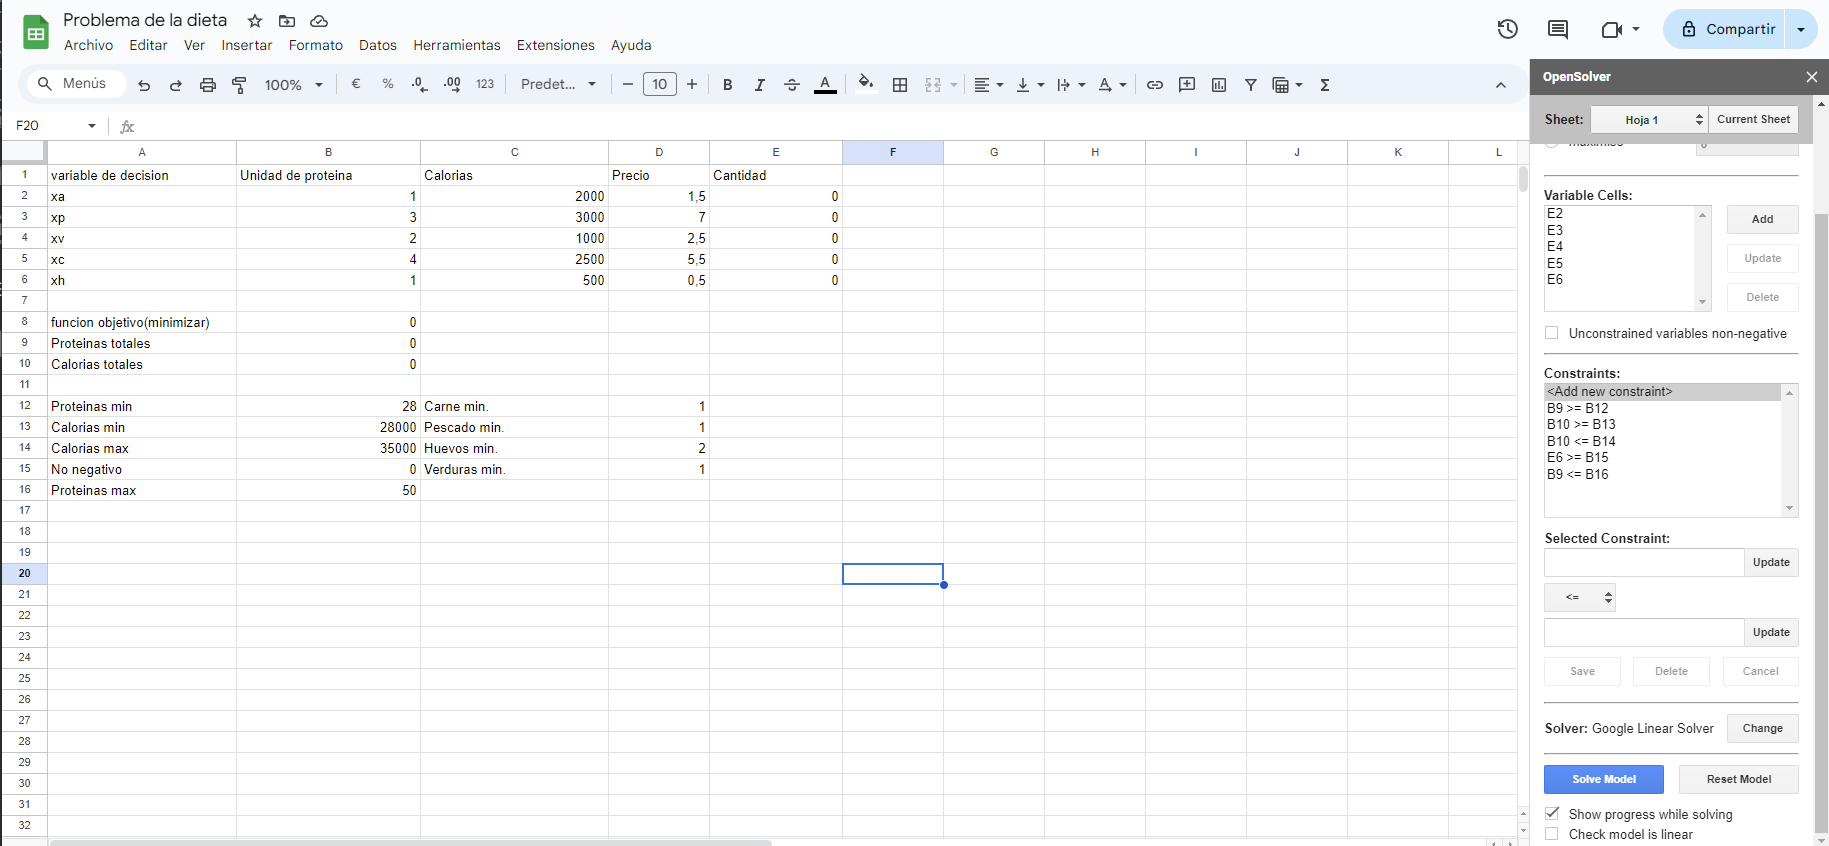
\includegraphics[width=.6\textwidth]{supuestoB.PNG}
    \label{fig:my_label}
\end{figure}

Lo mismo ha pasado con este supuesto.
\clearpage

\end{document}
